\section{Clustering}
\subsection{Übersicht}
\begin{figure}[h!]
	\centering
	\usetikzlibrary{trees}
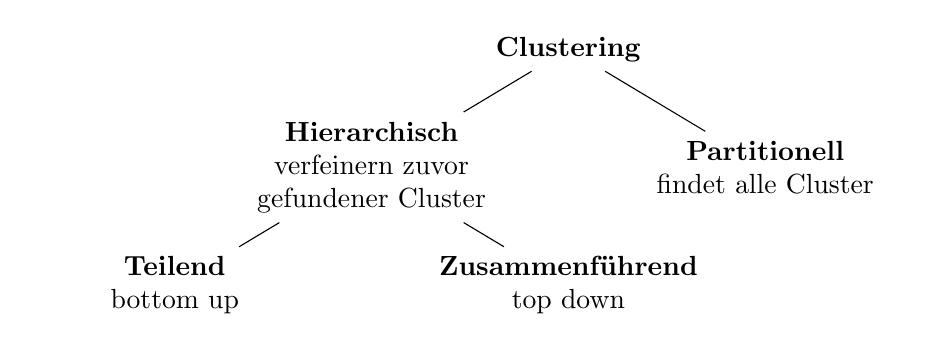
\begin{tikzpicture}[
	text width=3.5cm, align=flush center,
	level 1/.style={level distance=1.5cm, sibling distance=5cm},
	level 2/.style={}
]
	\node {\textbf{Clustering}}  % root {
		child { node {\textbf{Hierarchisch}\\verfeinern zuvor gefundener Cluster}
			child {node {\textbf{Teilend}\\ bottom up}}
			child {node {\textbf{Zusammenführend}\\ top down}}
		}
		child { node {\textbf{Partitionell} \\ findet alle Cluster} }
	;
\end{tikzpicture}

	\caption{Verschiedene Clustering Verfahren}
\end{figure}

\subsection{Distanzmasse}
Bevor man überhaupt clustern kann, benötigt man eine passende Distanzfunktion für die einzelnen Elemente untereinander und zu einem Cluster.
\begin{table}[h!]
	\centering
	\begin{tabularx}{\textwidth}{X| l }
		Beschreibung & Formel \\
		\hline
		{Der minimale Abstand zweier Elemente aus beiden Clustern (single linkage clustering)} & {
			$\underset{a \in A, b \in B}{min}\{d(a,b)\}$
		}
		\\
		{Der maximale Abstand zweier Elemente aus beiden Clustern (complete linkage clustering)} & {
			$\underset{a \in A, b \in B}{max}\{d(a,b)\}$
		}
		\\
		{Der durchschnittliche Abstand aller Elementpaare aus den beiden Clustern (average linkage clustering)} & {
			$\frac{1}{|A||B|} \sum\limits_{a \in A, b \in B}{d(a,b)}$
		}
		\\
		{Der durchschnittliche Abstand aller Elementpaare aus der Vereinigung von A und B (average group linkage)} & {
			$\frac{1}{|C|} \sum\limits_{x,y \in C, C=A \cup B}{d(x,y)}$
		}
		\\
		{Der Abstand der Mittelwerte der beiden Cluster (centroid method)} & {
			$d(\overline a, \overline b)$
		}
		\\
		{Die Zunahme der Varianz beim Vereinigen von A und B (Wards method)} & {
			$\frac{\overline a, \overline b}{\frac{1}{|A|} + \frac{1}{|B|}}$
		}
	\end{tabularx}
	\caption{Verschiedene Distanzmasse}
	\label{tab:distanzmasse}
\end{table}

\subsection{K-means Clustering}
Unüberwachtes hartes Clusteringverfahren welches nicht unbedingt konvergiert. Es ornet jeden Punkt demjenigen Cluster zu, dessen Mittelpunk ihm am nächsten liegt.
\begin{enumerate}
	\item Wahl der Anzahl Clusters k
	\item k Clusters erstellen (Mittelpunke zufällig wählen)
	\item Punkte den Clustern Zuordnen
	\item Berechnung der neuen Cluster-Schwerpunkte (Mittelpunkte)
	\item Wiederholung der letzten beiden Punkte bis ein Stabilitätsmerkmal erreicht ist
\end{enumerate}

\subsubsection{Nachteile}
\begin{itemize}
	\item Nicht immer das gleiche Ergebnis
	\item Muss nicht konvergieren
	\item Funkioniet nur gut bei gaussverteilten Haufen
\end{itemize}

\subsection{Ward-Clustering}
\begin{itemize}
	\item Bottom-up man begint mit einzelnen Objekten
	\item Immer die beiden ähnlichsten werden zusammengelegt
	\item Sobald genügend wenige Cluster übrigbleiben ist man fertig
\end{itemize}

\subsection{SCC- / Pott-Spin Clustering}
Es wird nicht vorgegeben wieviel Cluster erwartet werden. Pott-Spin verwendet Temperatur, SCS kann Cluster unterschiedlicher Dichte aufspüren.

